
\documentclass[Recitation9.tex]{subfiles}

\section{Optimal policy for a lock down}

\begin{frame}{Evaluating the lock down}
	Why are we stuck inside?
	\begin{itemize}
		\item Clearly, the policymakers thought this was the right choice;
		\item What does this mean for the implied value of a statistical life? (Benefits in terms of lives lost)
		\item What are we losing out of this? (Costs in terms of foregone consumption)
	\end{itemize}
\end{frame}


\begin{frame}{The trade-offs of a lock down}
Simple way to think about it (from Alvarez et al., 2020).
	\begin{itemize}
		\item Benefit: slower contagion rate $\Rightarrow$ less infected people at any given time $\Rightarrow$ hospitals are not overwhelmed $\Rightarrow$ less fatalities (for vulnerable age groups mostly?)
		\item Cost: lost output (for not infected and lost lives).
	\end{itemize}
The planner therefore wants to minimize the present discounted value of the following loss:
\[
	\underset{\text{wages lost}}{wL} + \underset{\text{deaths}}{I \phi(I)}\left[\underset{\text{lost production}}{\dfrac{w}{r}} + \underset{\text{extra loss}}{\chi}\right],
\]
where $I$ is the number of infected patients, and $\phi(I)$ is a fatality rate increasing in the number of infections (due to congested hospitals). The stock if infections, $I$, evolves according to an epidemiological SIR (susceptible-infected-recovered). If lock down is activated and effective, the rate of increase falls.
\end{frame}

\begin{frame}{It's all in the numbers!}
	\begin{figure}
		\caption{Baseline Parameters}
		\centering
		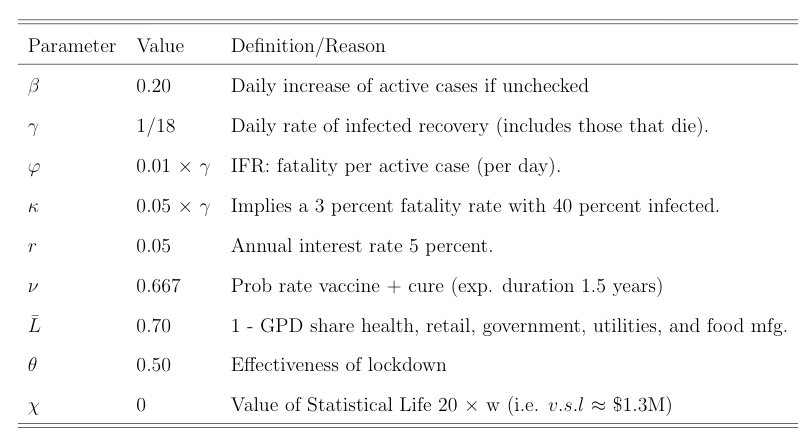
\includegraphics[width=0.7\linewidth]{Figures/AlvarezParameters}
		\label{fig:alvarez}
	\end{figure}
Plausible? My friend Gianluca Rinaldi estimated 0.05\% for the population below 60, and about 4\% above, so overall 1\% makes sense.
	
\end{frame}

\begin{frame}{Welfare gains from lock down}
\begin{figure}
	\centering
	\label{fig:alvarezgains}
	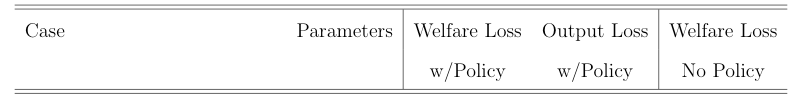
\includegraphics[width=0.7\linewidth]{Figures/AlvarezGains}\\
	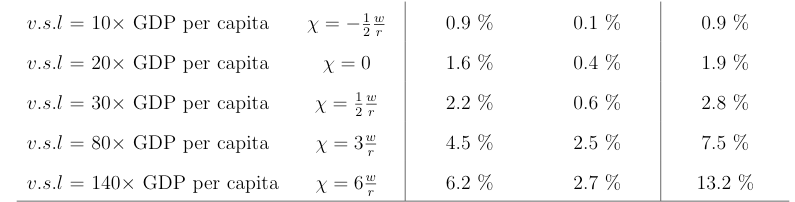
\includegraphics[width=0.7\linewidth]{Figures/AlvarezGains2}
\end{figure}
Benchmark assumes VSL is 20 times the GDP per capita in a year (about $\$1.3m$.)	The EPA suggests $\$7.4m$ of 2006 dollars, about $\$9.5m$ today, so for this look at last line. Using the EPA number, the gains in this model are about $7\%$ of annual GDP averted losses (pretty big!).
\end{frame}
\begin{frame}{What's missing?}
\begin{itemize}
	\item Heterogeneity by age: VSL varies a lot!
	\begin{figure}
		\centering
		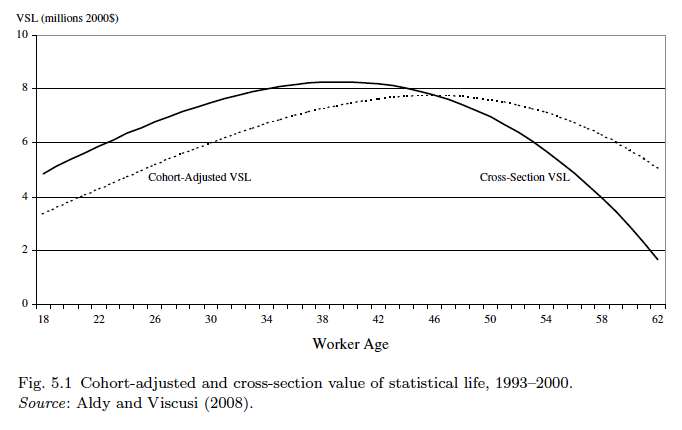
\includegraphics[width=0.4\linewidth]{Figures/ViscusiVSLCohort}
		\label{fig:viscusivslcohort}
	\end{figure}
	\item Hall et al. (2020) incorporate this fact and show that, on average, the US population would be willing to give about 20\% of annual consumption in order to avoid the COVID mortality \textit{overall}. 
\end{itemize}


\end{frame}


\begin{frame}{What's missing? Distributional issues!}
\begin{itemize}
	\item This is a ``representative agent'' model. Everyone gets the same utility and faces the same mortality.
	\item However, different \textit{labor market risks};
	\item In the US: job loss $\Rightarrow$ insurance loss $\Rightarrow$ \textit{higher health risk(!)}
	\item The model assumes economy bounces back right after\dots what about debt?
	\item Job prospects of incoming cohort?
	\item Next topic: job destroyed and costly to create $\Rightarrow$ labor market policies.
\end{itemize}
\end{frame}


\begin{frame}{Unemployment and search}
In this class, we have always assume that labor markets clear.
\begin{itemize}
	\item Crucial assumption: Everyone who wishes to work can get a job, every firm who wishes to fill a position does so instantly;
	\item Reality: both workers and firms \textit{search} for a match.
	\item Typical assumption:
	\[
		\text{matches} = m \cdot (\text{Number unemployed})^{\alpha} (\text{Number vacancies})^{1-\alpha}.
	\]
	\item Probability of entering a match for workers:
	\[
		\frac{\text{matches}}{\text{Number unemployed}} \  \Rightarrow \ \text{Falls with Unemployment}. 
	\]
	\item Many loose job at the same time $\Rightarrow$ long unemployment spells.
\end{itemize}


\end{frame}


\begin{frame}{The individual costs of destroying a match}
A large literature has found that losing a job has large, persistent effects for workers.
\begin{figure}
	\caption{From Jacobson et al. 1993}
	\centering
	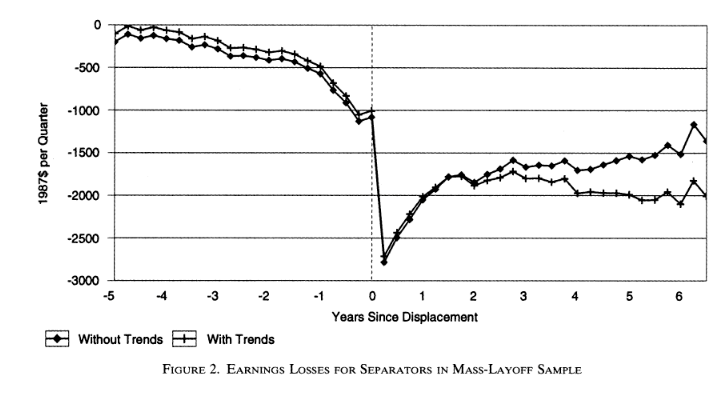
\includegraphics[width=0.5\linewidth]{Figures/EarningsLosses}
	\label{fig:earningslosses}
\end{figure}
Why? Loss of skills specific to the match (training received in the firm), loss of general human capital during unemployment.
\end{frame}



\begin{frame}{The social costs of destroying a match}
But that's not all\dots
\begin{itemize}
	\item In a recessions the many jobs that are destroyed will have to be recreated;
	\item Creating vacancies is costly (ads, agencies);
	\item Searching for a job is costly (time not spent otherwise);
	\item $\Rightarrow$ aggregate loss from unemployment crises;
	\item Partial mitigation: if there is a lot of unemployment, firms will open more vacancies \textit{ceteris paribus}. But what if recession affects their revenues and demand?
\end{itemize}
\end{frame}


\begin{frame}{The policy challenge}
How to best allocate funds to fight the impending recession? Labor market alternatives:
\begin{itemize}
	\item Boost unemployment benefits, so that demand does not fall as much (what US has done);
	\item Subsidize firms to keep workers and implement short-time work (STW), so that demand does not fall much \textit{and} the search costs post-recession are saved (what EU has done).
\end{itemize}
Requires these assumptions to be optimal:
\begin{itemize}
	\item US alternative: firms are optimally laying off, keeping the workers they will need after, thus partially internalizing the search costs to be borne later. Firms will not have long-term impact (survival not significantly affected now). Only friction is demand externality;
	\item EU: firms are often liquidity constrained, so they cannot keep their workers optimally. There is a labor market friction to correct.
\end{itemize}
\end{frame}

\begin{frame}{Differences in UI vs. STW across US and EU}
	\begin{figure}
		\caption{Giupponi and Landais, some weeks back (2020)}
		\centering
		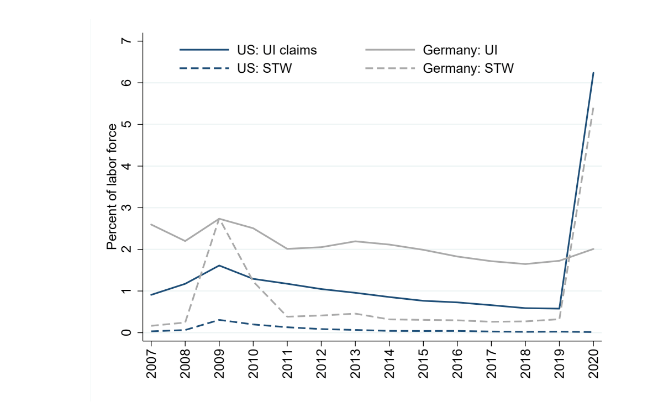
\includegraphics[width=0.5\linewidth]{Figures/GiupponiLandais}
		\label{fig:giupponilandais}
	\end{figure}
Quantitative estimates from Italy by Giupponi and Landais (2020) show that there are benefits over UI for short-term crises!
\end{frame}


\begin{frame}{Costs and benefits}
	So why did the US not do so?
	\begin{enumerate}
		\item Government actually believes markets operate efficiently. US labor market operates consistently better than the Italian one. Costs might not be worth the benefits.
		\item Costs/political concerns: UI benefit raise temporarily might cause less lobbying requests in the future compare to STW, afraid to introduce it;
		\item Related concern that it might become a more permanent policy: in the long-run, subsidizing jobs in crisis hampers reallocation across sectors.
	\end{enumerate}
\end{frame}

